\subsection{TODO}
\section{Lezione 2016-11-11}
% Insert what you need. Any row is associated with the improvment or mistake
% arise. In the first column you can insert what you should resolve or change,
% instead in the second column you may put the section where to apply some
% modification.
\begin{table}[H]
\begin{center}
\begin{tabular}{|p{\textwidth}|c|}
\hline
\multicolumn{1}{|c|}{\textbf{Miglioramento}} & \textbf{Sezione} \\ \hline
\end{tabular}
\end{center}
\caption{Tabella miglioramenti}
\label{tab:tab_todo}
\end{table}

\subsection{I Dataflow Framework}
I \textit{dataflow framework} sono un famiglia di algoritmi generici dove
estrarre informazioni dai programmi. Questi algoritmi vanno a risolvere quella
che viene chiamata \textit{dataflow analysis}.

I vari framework che si andranno a vedere serviranno per poter dedurre le
variabili vive, e quindi determinare i registri necessari, in base alle
relazioni tra i blocchi base.

Le relazioni vengono esposte tramite il \textit{Control Flow Graph}, dove i
vari blocchi base sono congiunti in base al prossimo possibile leader.

\begin{figure}[H]
  \centering
  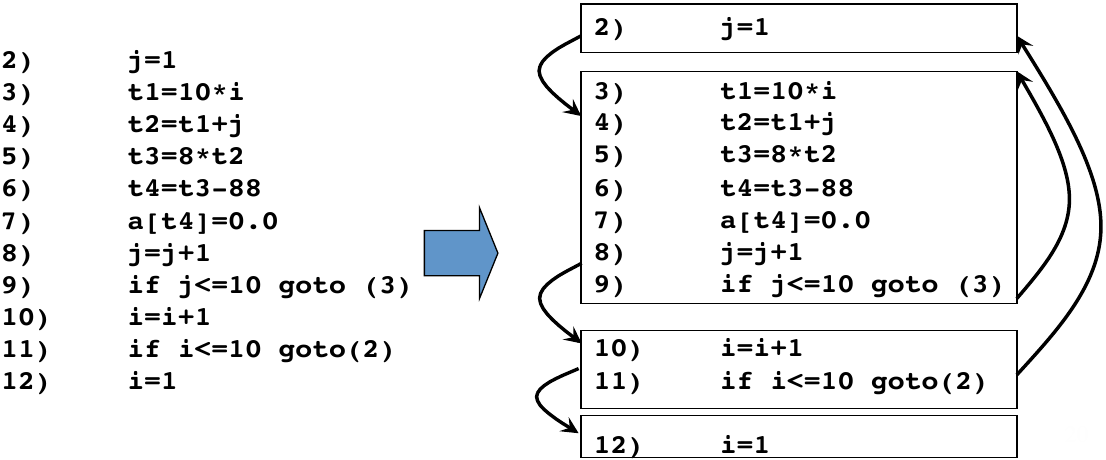
\includegraphics[scale=0.4]{res/image/control_flow_graph}
  \caption{Esempio \textit{Control Flow Graph}}
  \label{img:control_flow_graph}
\end{figure}

Noi possiamo considerare in modo sicuro un blocco per ogni istruzione,
omettendo il riquadro.

\begin{figure}[H]
  \centering
  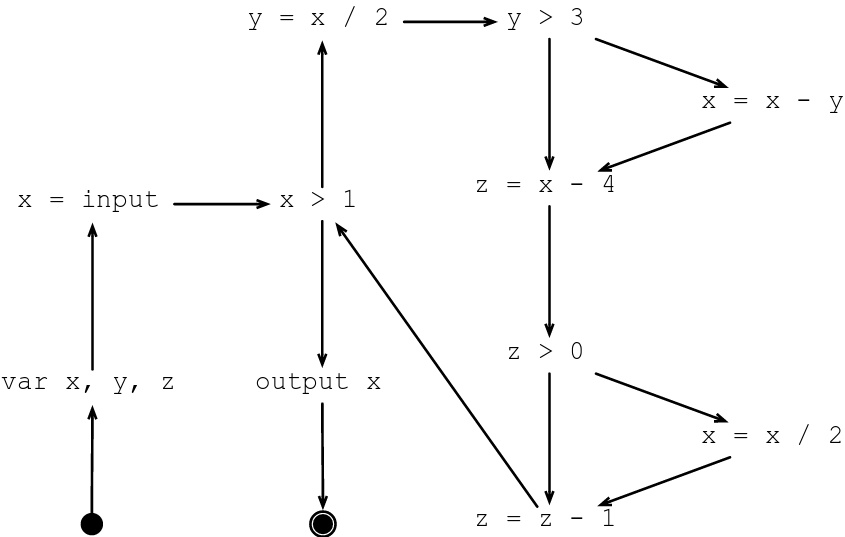
\includegraphics[scale=0.4]{res/image/cfg_no_block}
  \caption{Esempio \textit{Control Flow Graph} conclusivo}
  \label{img:cfg_no_block}
\end{figure}

Attraverso i vari framework si andr\'a a capire lo stato delle variabili
attraverso metodologie differenti. Tuttavia le fonti delle informazioni
rilevanti alle varie analisi sono uguali:

\paragraph{La \textit{origin information}}
dove l'informazione \`e ottenuta mediante immediata osservazione.
\paragraph{La \textit{propagation information}}
come l'informazione \`e passato lungo la sequenza d'istruzioni
('\textbf{locale}').
\paragraph{La \textit{joining information}}
come l'informazione \`e passato lungo i confini dei blocchi base
('\textbf{globale}').

\subsection{Liveness}
Dato il \textit{Control Flow Graph} bisogna capire quali insieme di variabili
sono vive in un istante punto del programma, in particolare tra i limite dei
blocchi base, dove nel grafo sono gli spigoli di congiunzione dei nodi.

\begin{figure}[H]
  \centering
  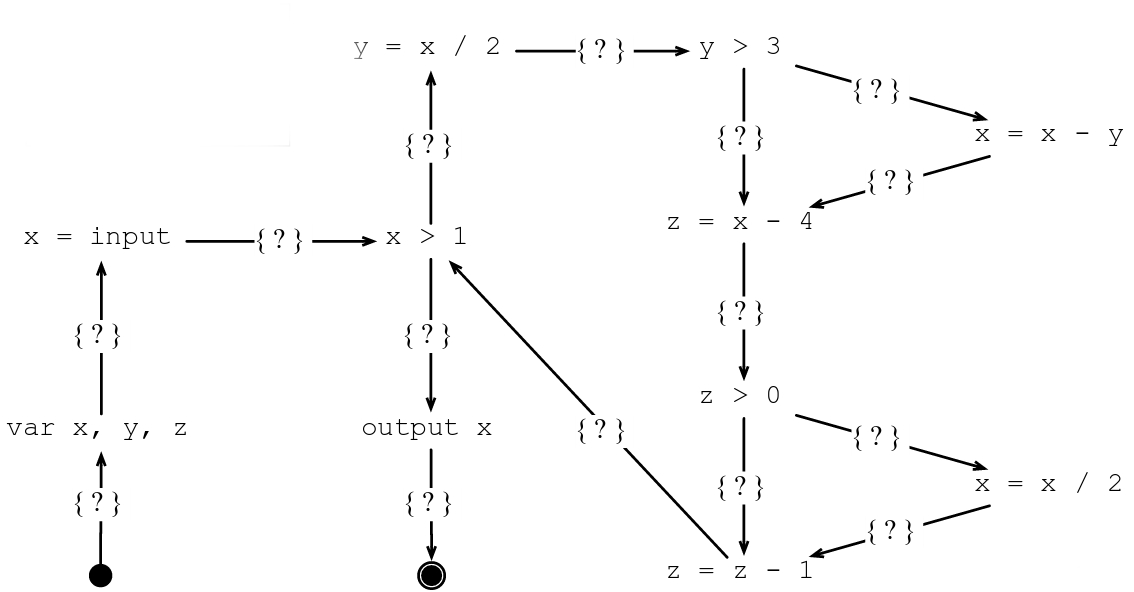
\includegraphics[scale=0.4]{res/image/cfg_liveness}
  \caption{Come determinare l'insieme delle variabili vive?}
  \label{img:cfg_liveness}
\end{figure}

\begin{definition}[Alive Variable]
Se noi assumiamo un infinito insieme di registri allora la variabile $v$
dovrebbe essere in un registro nel punto del programma $p$ se:
\begin{enumerate}
\item esiste una path $P$ da $p \to p_u$ dove $v$ \`e usata
\item $P$ non incluse istruzioni dove $v$ \`e definita
\end{enumerate}

Le due condizione determinano quando $v$ \`e \textbf{viva} nel programma.
\end{definition}

\begin{figure}[H]
  \centering
  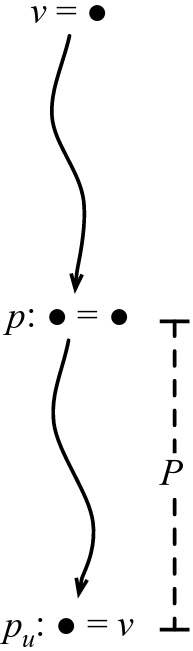
\includegraphics[scale=0.4]{res/image/liveness_v}
  \caption{Percorso dove $v$ \`e viva}
  \label{img:liveness_v}
\end{figure}

\subsubsection{Origin Information}
Se una variabile \`e usata al punto $p$ del programma, allora deve essere via
\textbf{immediatamente prima} di $p$.

\begin{figure}[H]
  \centering
  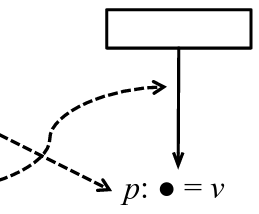
\includegraphics[scale=0.4]{res/image/origin_liveness}
  \caption{La \textit{origin information} per \textit{liveness}}
  \label{img:origin_liveness}
\end{figure}

\subsubsection{Propagation Information}
Una variabile \`e viva \textbf{immediatamente prima} di un punto $p$ del
programma, sse:
\begin{itemize}
\item \'E viva immediatamente prima di $p$
\item Non viene ridefinita in $p$
\end{itemize}

oppure \textbf{viene usata in} $p$.

\begin{figure}[H]
  \centering
  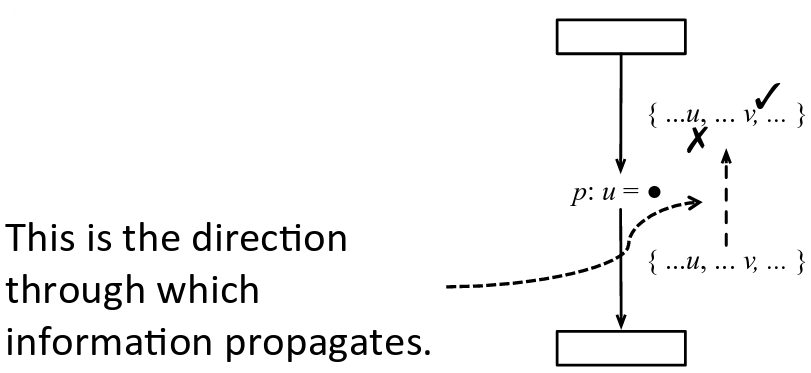
\includegraphics[scale=0.4]{res/image/propagation_liveness}
  \caption{La \textit{propagation information} per \textit{liveness}}
  \label{img:propagation_liveness}
\end{figure}

Si noti che la propagazione di fig.\ref{img:propagation_liveness} avviene verso
il padre in quanto non soddisfa il punto 2. Il fenomeno deriva che la
definizione dichiara quando una variabile \`e viva \textbf{prima} di $p$ usando
informazioni \textbf{attuale} o \textbf{successiva}.

\subsubsection{Joining Information}
Se la variabile $v$ \`e viva \textbf{immediatamente prima} ogni predecessore di
$p$, allora deve essere viva \textbf{immediatamente dopo} $p$.

\begin{figure}[H]
  \centering
  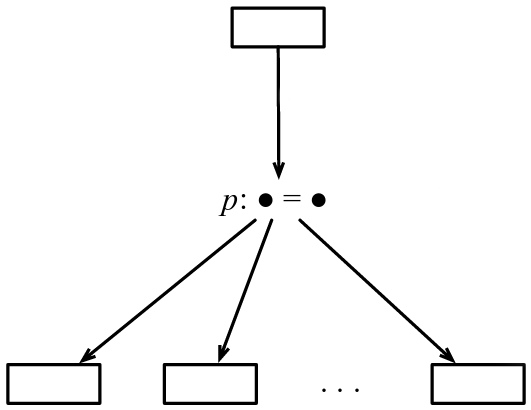
\includegraphics[scale=0.4]{res/image/joining_liveness}
  \caption{La \textit{joining information} per \textit{liveness}}
  \label{img:joining_liveness}
\end{figure}

\subsubsection{IN e OUT}
Ad ogni punto del programma $p$ associamo due insiemi:
\begin{align*}
& IN =
\{\text{variabili che vive immediatamente \textbf{prima} di $p$}\}
\\
& OUT =
\{\text{varaibili che vive immediatamente \textbf{dopo} di $p$}\}
\end{align*}

\begin{figure}[H]
  \centering
  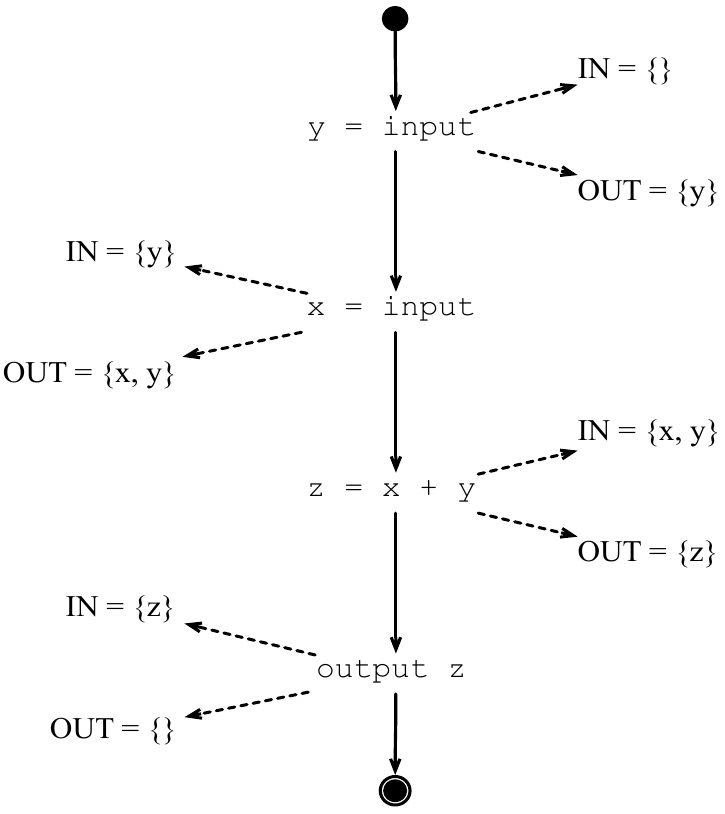
\includegraphics[scale=0.4]{res/image/in_out}
  \caption{Insieme IN e OUT per \textit{liveness}}
  \label{img:in_out}
\end{figure}

Definiamo l'equazioni. Dato il punto $p$ del programma con l'istruzione $v=E$
gli insiemi $IN$ e $OUT$ sono definiti come segue:
\begin{align*}
p : v = E &                                             \\
          & IN(p) = (OUT(p)\setminus\{v\}) \cup vars(E) \\
          & OUT(p) = \bigcup IN(p_s), p_s \in succ(p)
\end{align*}

Abbiamo aggiunto due funzioni: $vars(E)$, l'insieme delle variabili in $E$, e
$succ(p)$, l'insieme di nodi del CFG successori di $p$.

\subsubsection{Risultato}
\begin{figure}[H]
  \centering
  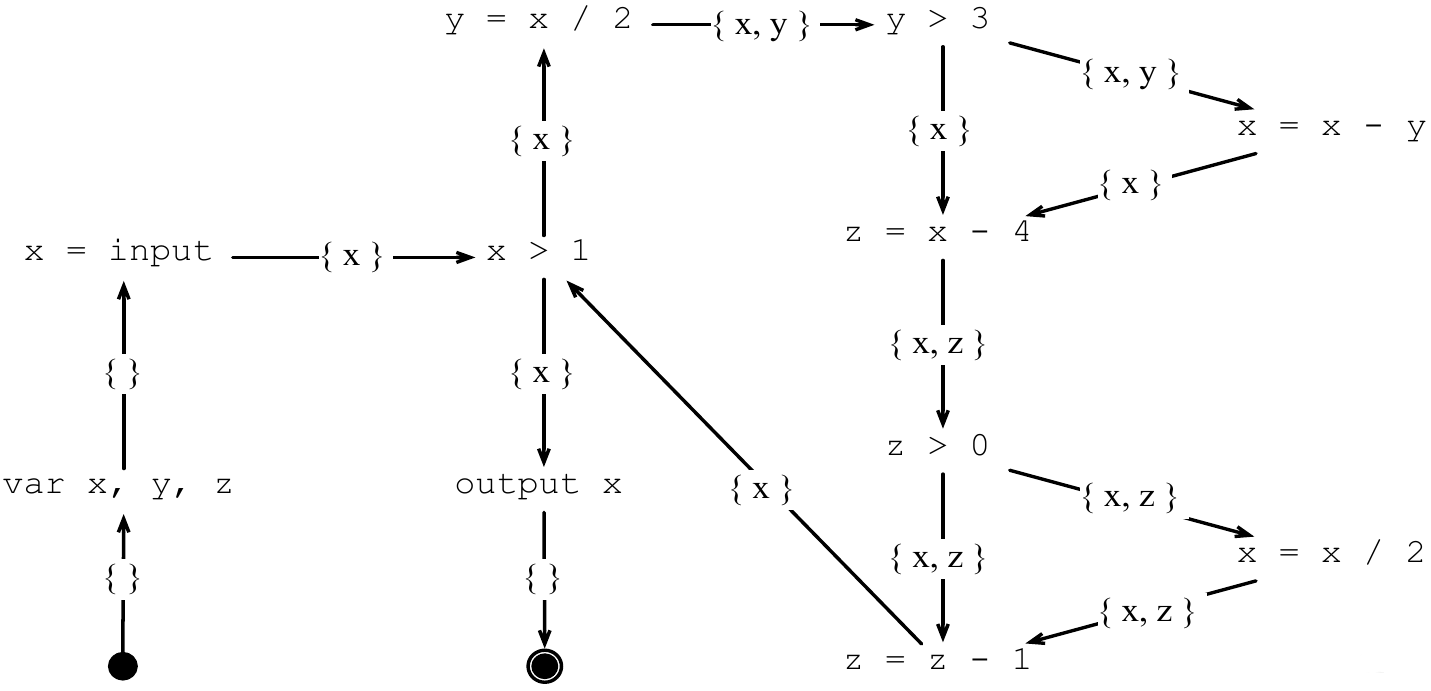
\includegraphics[scale=0.4]{res/image/example_liveness}
  \caption{Risultato del \textit{liveness} framework}
  \label{img:example_liveness}
\end{figure}

\subsection{Available Expression}
La \textit{available expression} mira a eliminare le computazioni eseguite
pi\`u volte all'interno del programma.

\begin{figure}[H]
  \centering
  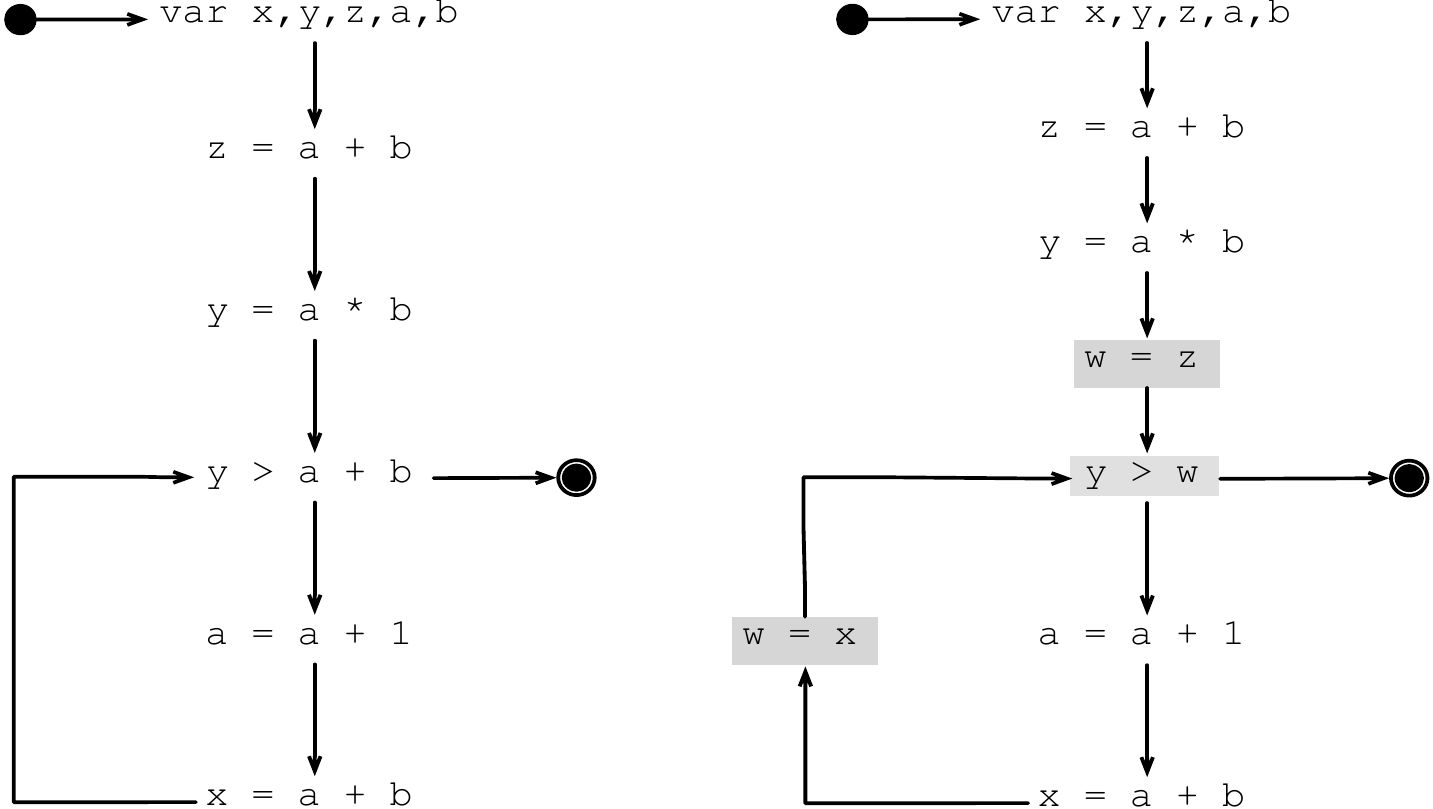
\includegraphics[scale=0.35]{res/image/redundant_sum}
  \caption{Esempio eliminazione somme ridondanti}
  \label{img:redundant_sum}
\end{figure}

Per ottenere il miglioramento di figura sopra, bisogna sapere quali espressioni
sono disponibili in un certo punto in modo da rimuovere i duplicati.

\begin{definition}[Available Expression]
Un'espressione \`e disponibile ad un punto del programma se il suo valore
\textbf{corrente} \`e gi\`a stato computato prima dell'esecuzione
\end{definition}

\subsubsection{Origin Information}
Se una variabile \`e usata al punto $p$, allora \`e disponibile
\textbf{immediatamente dopo} $p$, purch\'e $p$ non ridefinisce nessuna delle
variabili che l'espressione usa.

\begin{figure}[H]
  \centering
  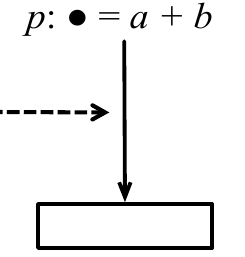
\includegraphics[scale=0.4]{res/image/origin_available}
  \caption{La \textit{origin information} per \textit{available}}
  \label{img:origin_available}
\end{figure}

\subsubsection{Propagation Information}
Un espressione $E$ \`e disponibile \textbf{immediatamente dopo} di un punto $p$
del programma sse:
\begin{enumerate}
\item \`E immediatamanete disponbile prima di $p$
\item Nessuna variabile di $E$ \`e ridefinita in $p$
\end{enumerate}

oppure:
\begin{enumerate}
\item \`E usata in $p$
\item Nessuna variabile di $E$ \`e ridefinita in $p$
\end{enumerate}

\begin{figure}[H]
  \centering
  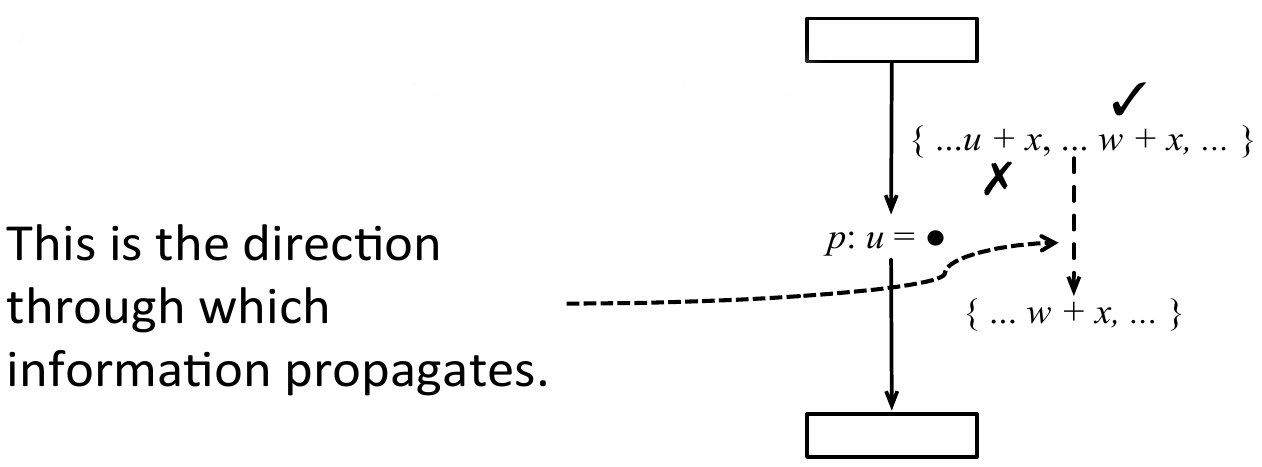
\includegraphics[scale=0.4]{res/image/propagation_available}
  \caption{La \textit{propagation information} per \textit{available}}
  \label{img:propagation_available}
\end{figure}

\subsubsection{Join Information}
Se un'espressione $E$ \`e disponibile \textbf{immediatamente dopo} ogni
predecessore di $p$, allora deve essere disponibile
\textbf{immediatamente prima} di $p$.

\begin{figure}[H]
  \centering
  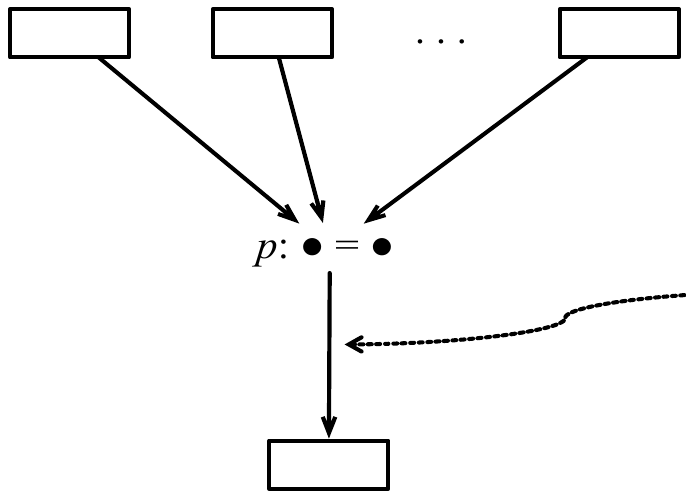
\includegraphics[scale=0.4]{res/image/joining_available}
  \caption{La \textit{joining information} per \textit{available}}
  \label{img:joining_available}
\end{figure}

\subsubsection{IN e OUT}
Per risolvere l'analisi delle espressioni disponibili, associamo ad ogni
punto $p$ del programma due insieme:
\begin{align*}
& IN =
\{\text{esperssioni disponibili \textbf{immediatamente prima} di $p$}
\} \\
& OUT =
\{\text{espressioni disponibili \textbf{immediatamente dopo} di $p$}
\}
\end{align*}

\begin{figure}[H]
  \centering
  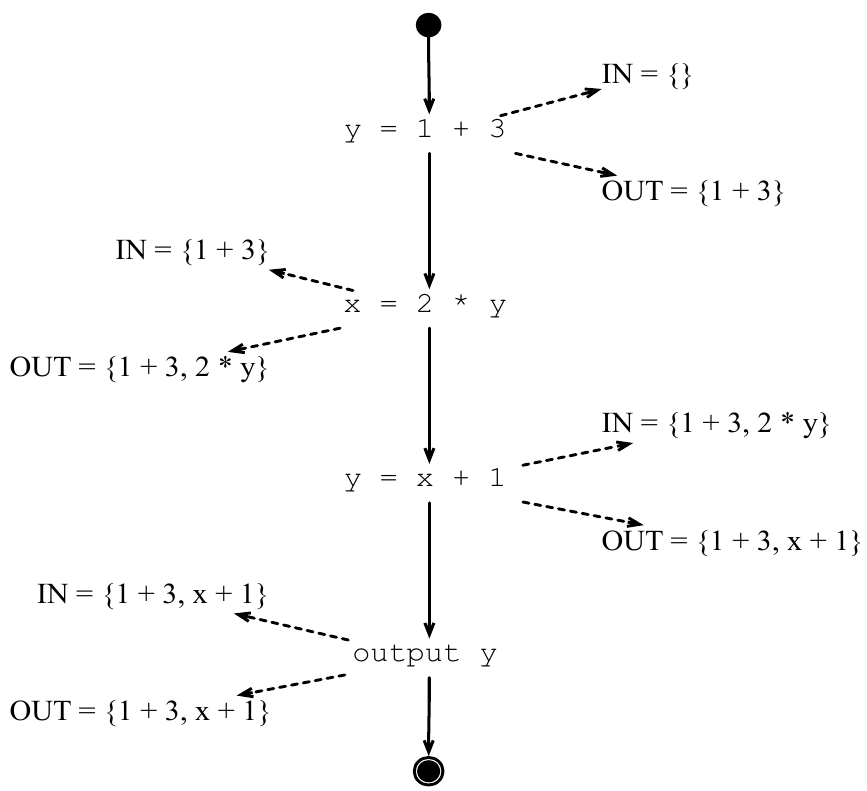
\includegraphics[scale=0.4]{res/image/in_out_available}
  \caption{Insiemi IN e OUT per \textit{liveness}}
  \label{img:in_out_available}
\end{figure}

Definiamo l'equazione. Dato il punto $p$ del programma con l'istruzione $v=E$,
gli insiemi $IN$ e $OUT$ sono definit come segue:
\begin{align*}
p : v = E &                                               \\
          & IN(p) = \bigcap OUT(p_s), p_s \in pred(p)     \\
          & OUT(p) = (IN(p) \cup E) \setminus Expr(v)
\end{align*}

Abbiamo aggiunto due funzioni: $pred(p)$, l'insieme dei nodi del CFG preceduti
da $p$, e $Expr(v)$, l'insieme d'istruzioni che usano $v$.

\subsubsection{Risultato}
\begin{figure}[H]
  \centering
  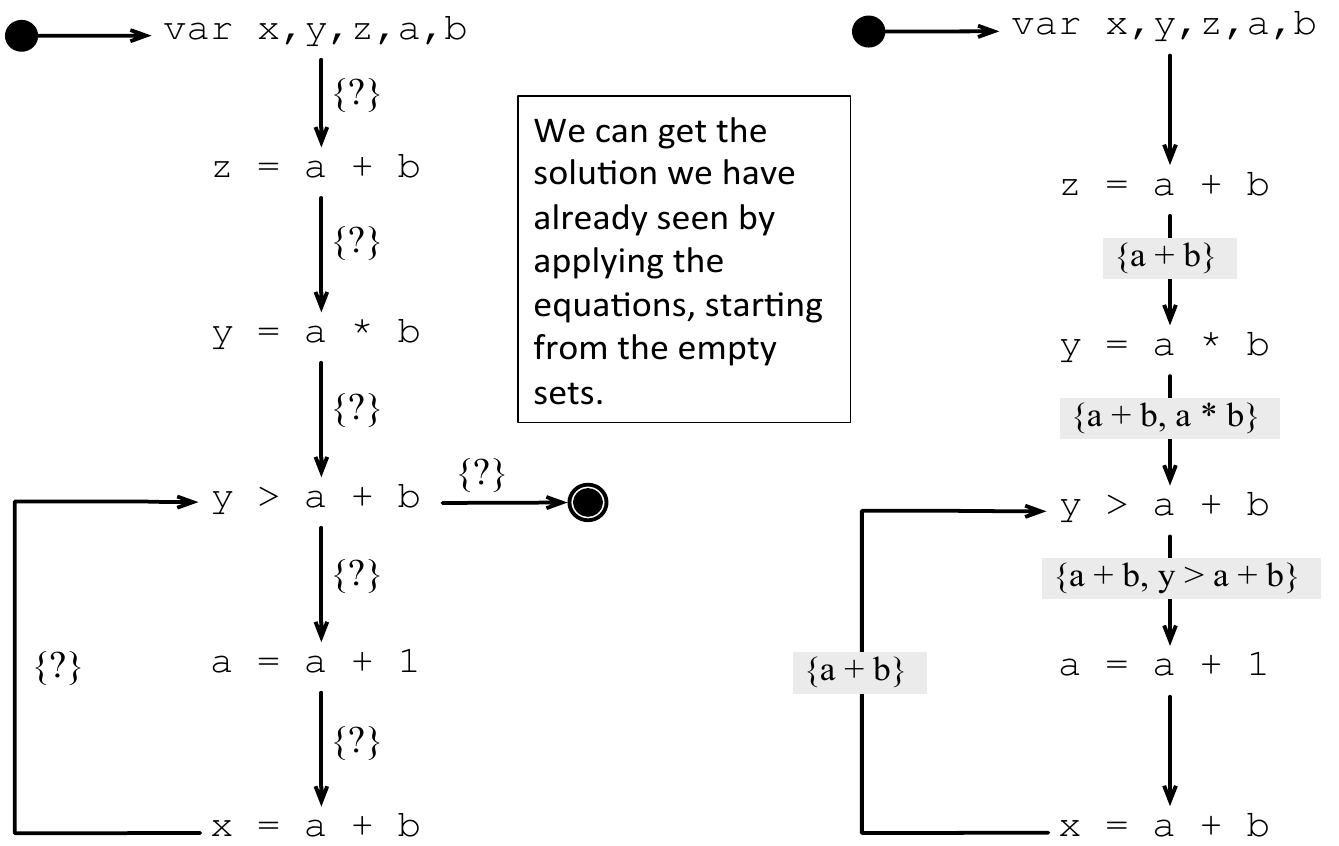
\includegraphics[scale=0.4]{res/image/example_available}
  \caption{Risultato del \textit{available} framework}
  \label{img:example_available}
\end{figure}

\subsection{Very Busy Expression}
La \textit{very busy expression} mira a calcolare una sola volta tutte quelle
espressioni in un branch decisionale che sono indipendenti dal risultato della
guardia. In altre parole, se un'espressione ha lo stesso valore in tutti i
rami, basta spostare la sua computazione prima di entrare nel costrutto logico
e riutilizzarlo quando richiesto.

\begin{figure}[H]
  \centering
  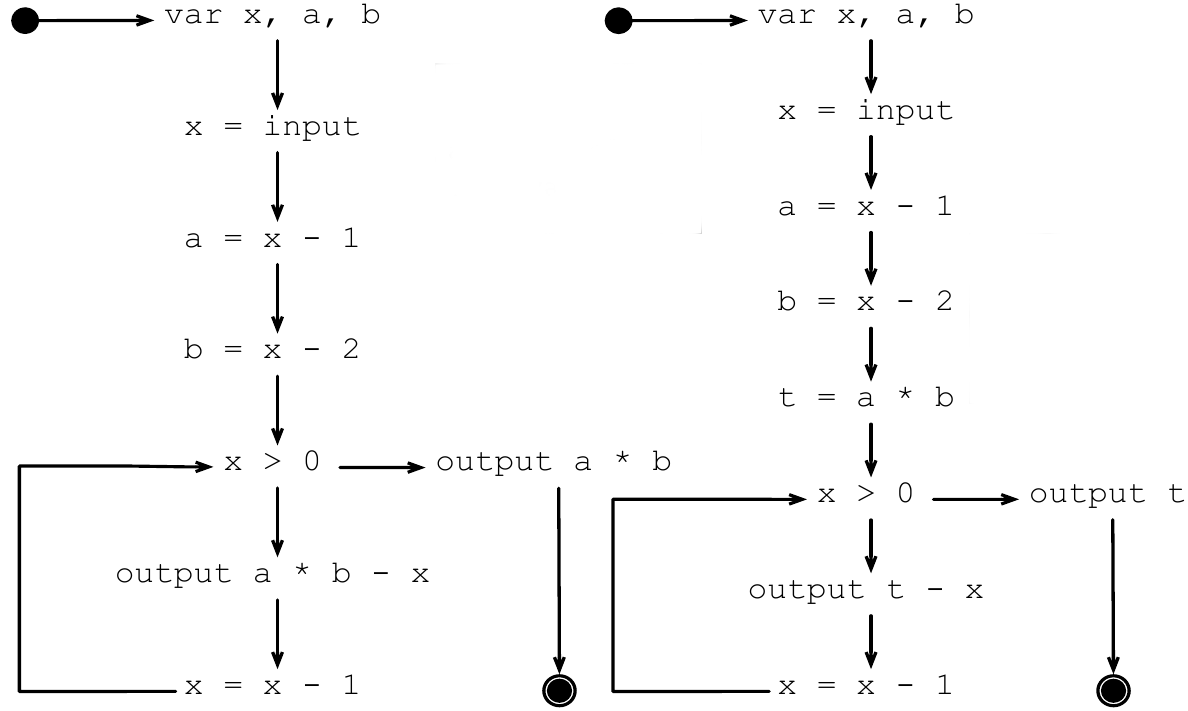
\includegraphics[scale=0.4]{res/image/indipendent_path}
  \caption{Calcolo espressione indipendente dalla ramo}
  \label{img:indipendent_path}
\end{figure}

Per ottenere il miglioramento sopra bisogna sapere che $a*b$ era una
\textit{very busy expression} prima di entrare nel loop.

\begin{definition}[Very Busy Expression]
Un'espressione \`e \textit{very busy} ad un punto del programma se verr\'a
computata prima della terminazione del programma lungo \textbf{ogni percorso}
a partire dalla fine fino al punto del programma.
\end{definition}

\subsubsection{Origin Information}
Se un'espressione \`e usata al punto $p$, allora \`e \textit{very busy}
\textbf{immediatamente prima} di $p$.

\begin{figure}[H]
  \centering
  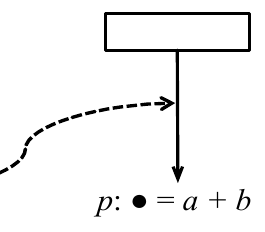
\includegraphics[scale=0.4]{res/image/origin_very-busy}
  \caption{La \textit{origin information} per \textit{very bust}}
  \label{img:orgin_very-busy}
\end{figure}

\subsubsection{Propagation Information}
Un espressione $E$ \`e \textit{very busy} \textbf{immediatamente prima} di $p$
sse:
\begin{enumerate}
\item \`E \textit{very busy} \textbf{immediatamente dopo} $p$
\item Nessuna variabile di $E$ \`e definita in $p$
\end{enumerate}

oppure l'espressione $E$ \`e usata in $p$.

\begin{figure}[H]
  \centering
  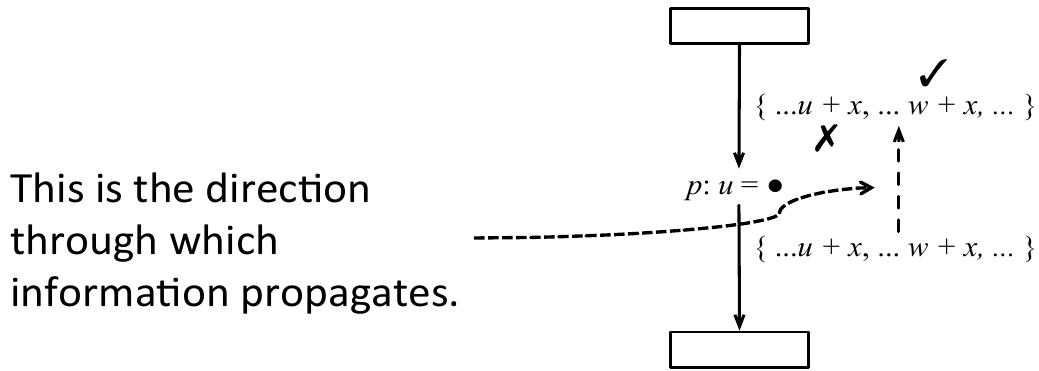
\includegraphics[scale=0.4]{res/image/propagation_very-busy}
  \caption{La \textit{propagation information} per \textit{very busy}}
  \label{img:propagation_very-busy}
\end{figure}

\subsubsection{Joining Information}
Se un'espressione $E$ \`e \textit{very busy} \textbf{immediatamente prima} di
ogni successore di $p$, allora deve essere \textit{very busy}
\textbf{immediatamente dopo} $p$.

\begin{figure}[H]
  \centering
  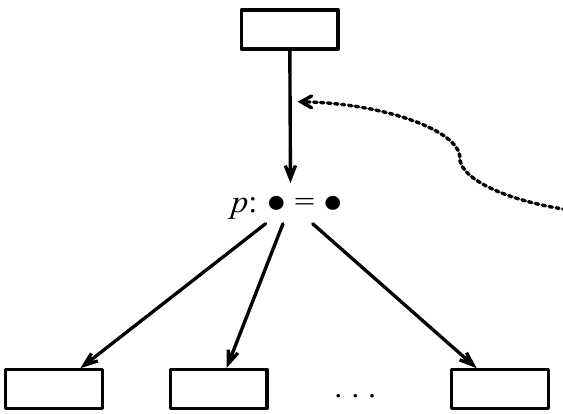
\includegraphics[scale=0.4]{res/image/joining_very-busy}
  \caption{La \textit{joining information} per \textit{very busy}}
  \label{img:joining_very-busy}
\end{figure}

\subsubsection{IN e OUT}
Per risolvere l'analisi dell'espressioni \textit{very busy}, associamo ad ogni
punto del programma $p$ due insiemi:
\begin{align*}
& IN = \{
\text{espressioni \textit{very busy} \textbf{immeditamente prima} di $p$}
\} \\
& OUT = \{
\text{espressioni \textit{very busy} \textbf{immeditamente dopo} di $p$}
\}
\end{align*}

\begin{figure}[H]
  \centering
  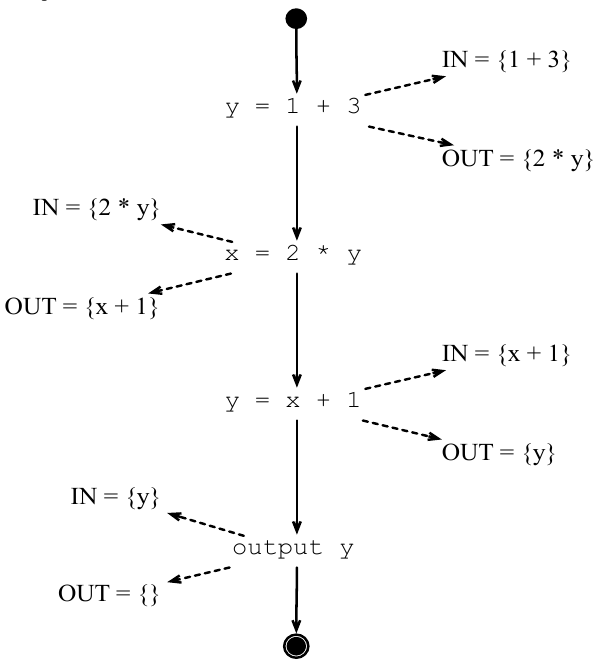
\includegraphics[scale=0.4]{res/image/in_out_very-busy}
  \caption{Insiemi $IN$ e $OUT$ per \textit{very busy}}
  \label{img:in_out_very-busy}
\end{figure}

Definiamo l'equazioni. Dato il punto del programma $p$ l'espressione $v=E$, gli
insiemi $IN$ e $OUT$ sono definiti come segue:
\begin{align*}
p: v = E &                                               \\
         & IN(p) = (OUT(p) \setminus Expr(v)) \cup \{E\} \\
         & OUT(p) = \bigcap IN(p_s), p_s \in succ(p)
\end{align*}

Abbiamo aggiunto due funzioni: $succ(p)$, l'insieme dei nodi del CFG che sono
successori di $p$, e $Expr(v)$, l'insieme d'istruzioni che usano $v$.

\subsubsection{Risultato}
\begin{figure}[H]
  \centering
  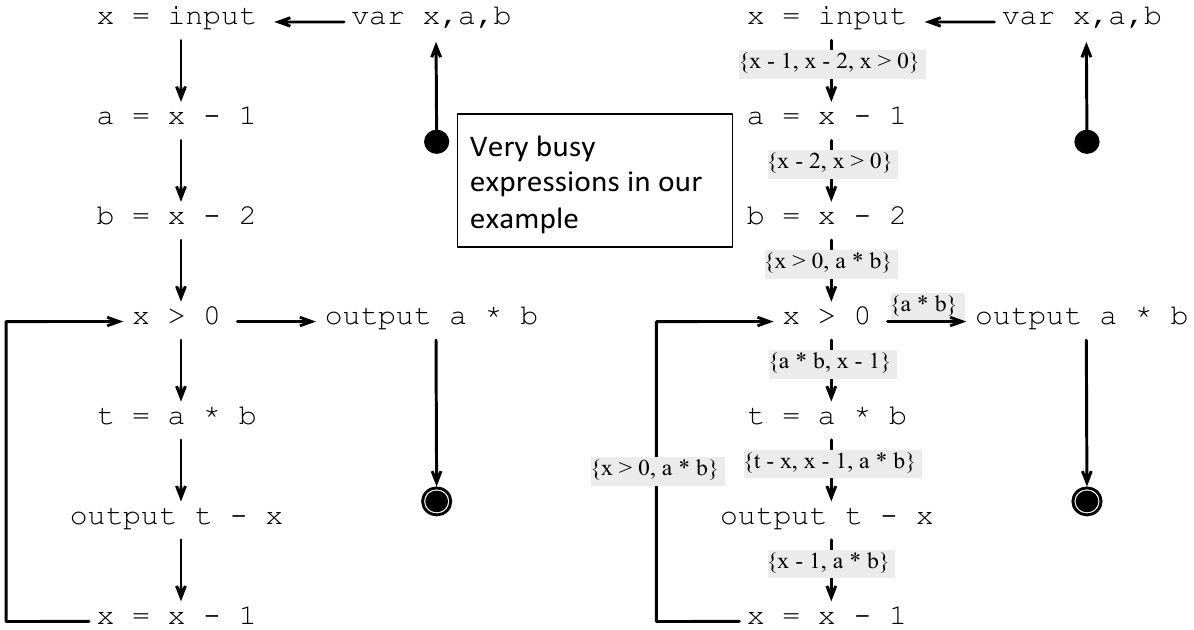
\includegraphics[scale=0.4]{res/image/example_very-busy}
  \caption{Risultato della \textit{very busy}}
  \label{img:example_very-busy}
\end{figure}

All'ingresso del loop \`e \textbf{sicuro} spostare il calcolo di $a*b$ perch\'e
non forziamo il programma ha fare \textbf{nessun lavoro extra} in ogni
circostanza.

\subsection{Reaching Definition}
La \textit{reaching definition} mira ad eliminare tutte le \textbf{definizioni
morte} ovvero quelle espressioni dove la definizione di una variabile non
raggiunge nessun uso di questa variabile.

\begin{figure}[H]
  \centering
  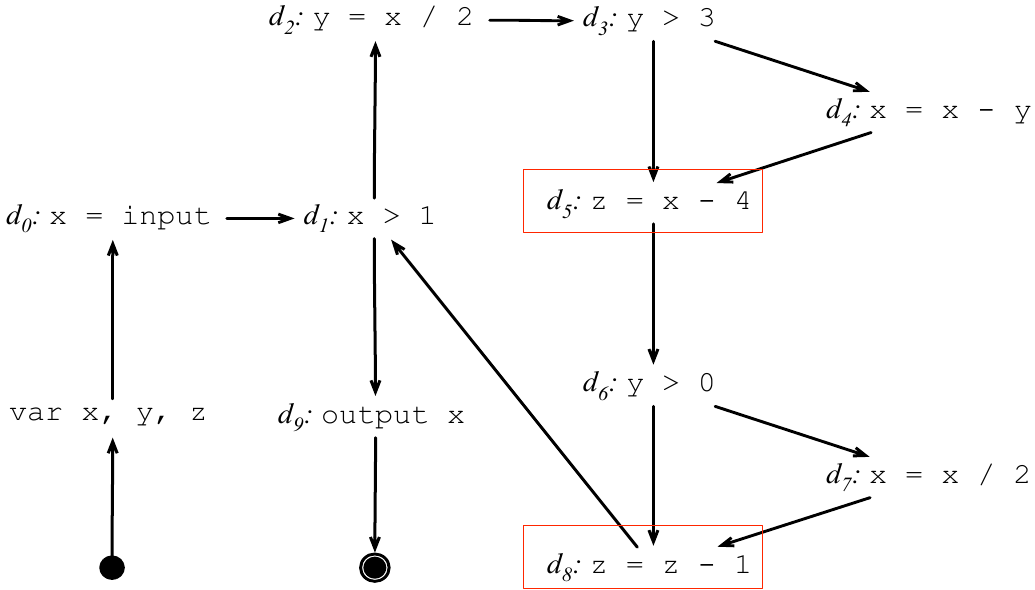
\includegraphics[scale=0.4]{res/image/dead_definition}
  \caption{Evidenziazione delle istruzioni morte nel CFG}
  \label{img:dead_definition}
\end{figure}

\begin{definition}[Reaching Definition]
Una definizione di una variabile $v$, al punto del programma $p$, raggiunge un
punto $p'$ del programma, se c'\`e un percorso $p \to p'$ in cui non si
incontrano altre definizioni di $v$.
\end{definition}

\begin{figure}[H]
  \centering
  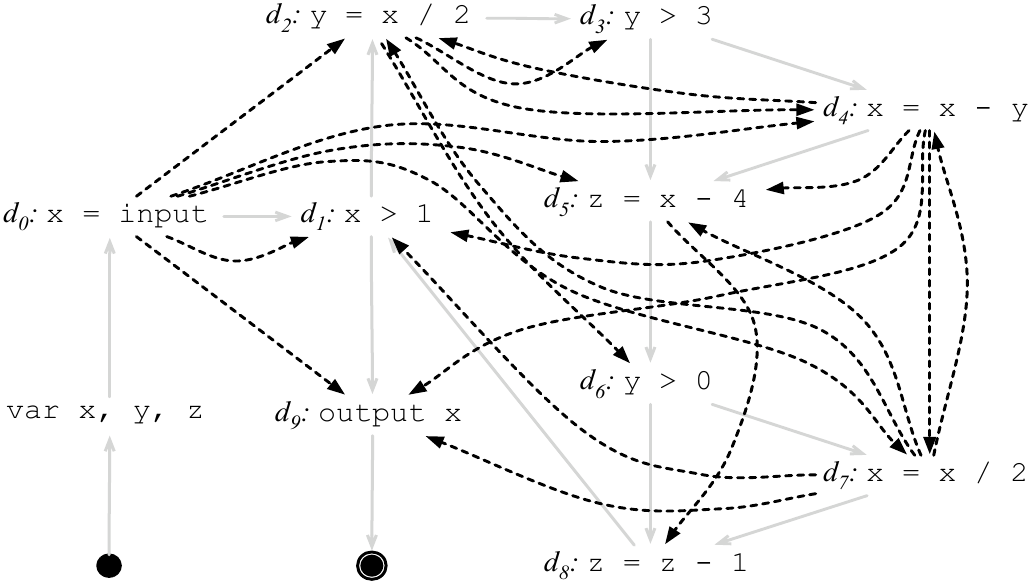
\includegraphics[scale=0.4]{res/image/show_path_use}
  \caption{Percorsi delle definizioni nel CFG}
  \label{img:show_path_use}
\end{figure}

\subsubsection{Origin Information}
Se un punto del programma $p$ definisce una variabile $v$, allora $v$ raggiunge
il punto \textbf{immediatamente dopo} $p$.

\begin{figure}[H]
  \centering
  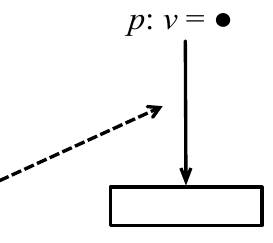
\includegraphics[scale=0.4]{res/image/origin_reaching}
  \caption{La \textit{origin information} di \textit{reaching}}
  \label{img:origin_reaching}
\end{figure}

\subsubsection{Propagation Information}
Una definizione di una variabile $v$ raggiunge il punto del programma
\textbf{immediatamente dopo} $p$, sse:
\begin{enumerate}
\item La definizione raggiunge il punto \textbf{immediatamente prima} di $p$
\item La variabile $v$ non \`e ridefinita in $p$
\end{enumerate}

oppure la variabile $v$ \`e ridefinita in $p$.

\begin{figure}[H]
  \centering
  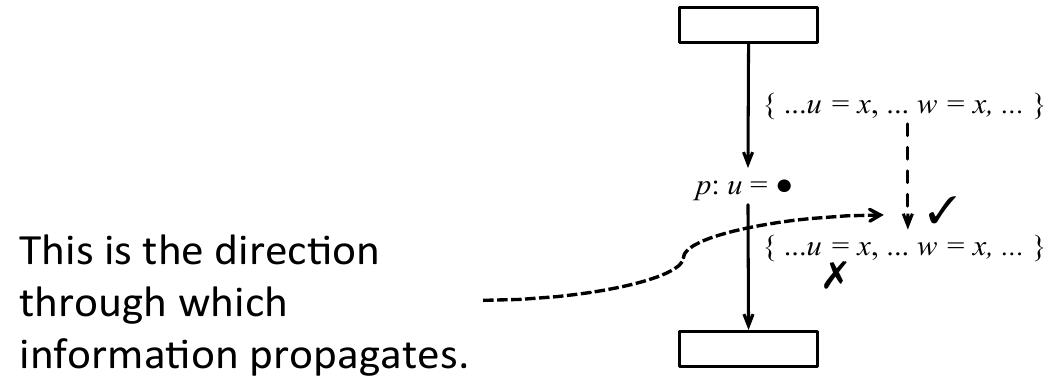
\includegraphics[scale=0.4]{res/image/propagation_reaching}
  \caption{La \textit{propagation information} di \textit{reaching}}
  \label{img:propagation_reaching}
\end{figure}

\subsubsection{Joining Information}
Se la definizione di una variabile $v$ raggiunge il punto
\textbf{immediatamente dopo} almeno un predecessore di $p$, allora raggiunge il
punto \textbf{immediatamente prima} di $p$.

\begin{figure}[H]
  \centering
  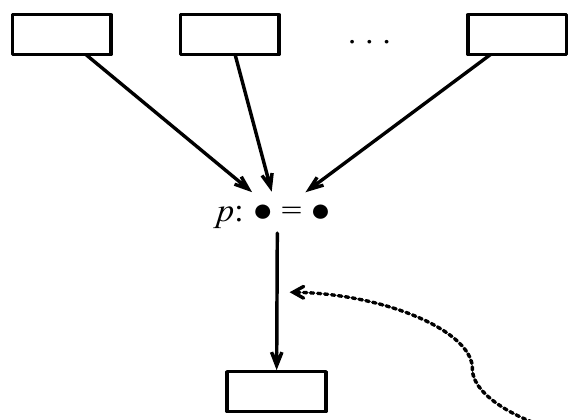
\includegraphics[scale=0.4]{res/image/joining_reaching}
  \caption{La \textit{joining information} di \textit{reaching}}
  \label{img:joining_reaching}
\end{figure}

\subsubsection{IN e OUT}
Per risolvere l'analisi delle \textit{reaching definition}, associamo ad ogni
punto del programma $p$ due insiemi:
\begin{align*}
& IN = \{
\text{
definizioni che raggiungono il punto \textbf{immediatamente prima} di $p$
}
\} \\
& OUT = \{
\text{definizioni che raggiungono il punto \textbf{immediatamente dopo} $p$}
\}
\end{align*}

\begin{figure}[H]
  \centering
  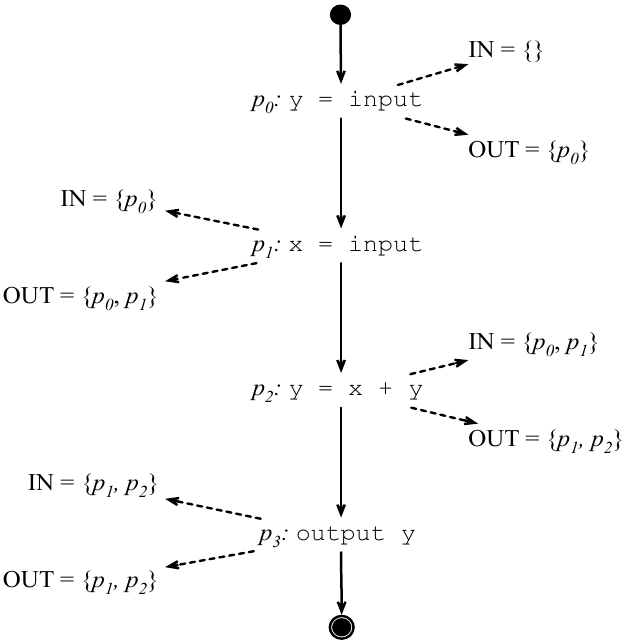
\includegraphics[scale=0.4]{res/image/in_out_reaching}
  \caption{Gli insiemi $IN$ e $OUT$ di \textit{reaching}}
  \label{img:in_out_reaching}
\end{figure}

Definiamo l'equazioni. Dato un punto del programma $p$ in cui \`e definita
l'istruzione $v = E$, definiamo gli insieme $IN$ e $OUT$ come segue:
\begin{align*}
p: v = E &                                                   \\
         & IN(p) = \bigcup OUT(p_s), p_s \in pred(p)         \\
         & OUT(p) = (IN(p) \setminus defs(v)) \cup \{p\}
\end{align*}

Abbiamo aggiunto due funzioni: $pred(p)$, l'insieme dei nodi del CFG che sono
predecessori di $p$, e $defs(v)$, l'insieme delle definizioni di $v$ nel
programma.

\subsubsection{Risultato}
\begin{figure}[H]
  \centering
  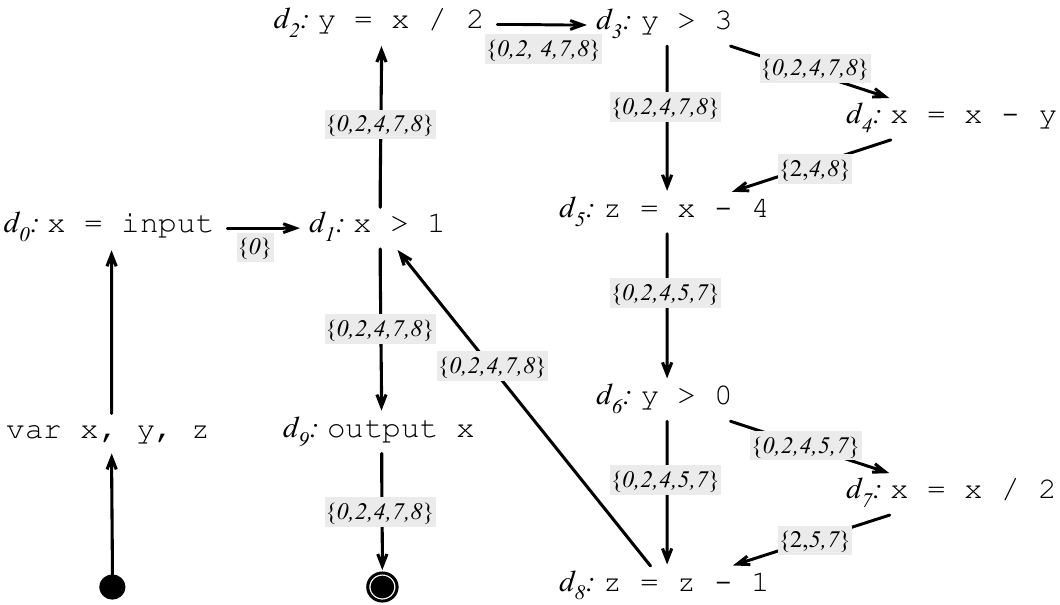
\includegraphics[scale=0.4]{res/image/example_reaching}
  \caption{Risultato della \textit{reaching}}
  \label{img:example_reaching}
\end{figure}

\subsection{Nota generale calcolo IN e OUT}
In caso di \textbf{ciclo} entrarci con gli $IN$ e $OUT$ che si hanno gi\`a,
ovvero quelli calcolati fino al figlio in cui si \`e entrati. Durante
l'attraversamento verranno trovati i nuovi $IN$ e $OUT$. Quando si \`e
ritornati alla guarda riapplicare le regole con gli insieme aggiornati. Ora
il punto $p$ dell'ingresso del ciclo ha i due insieme corretti ma il resto del
corpo no, rientrare nel ciclo per calcolare gli $IN$ e $OUT$ con le
informazioni aggiornate. Quando si torner\'a alla guarda per la seconda volta,
tutto sotto CFG del ciclo sar\'a configurato correttamente.

\subsection{Ricerca dei fattori comuni}
Le quattro tipi d'analisi viste hanno dei punti in comune il quale permette la
categorizzazione in altrettante metodi d'analisi:
\paragraph{May Analysis}
Si tiene traccia dei fatti che \textbf{potrebbero} succedere durante
l'esecuzione del programma.
\paragraph{Must Analysis}
Si tiene traccia dei fatti che \textbf{succederanno} (con certezza) durante
l'esecuzione del programma.
\paragraph{Backward Analysis}
L'informazione viene propagata nella direzione \textbf{opposta} al flusso del
programma.
\paragraph{Forward Analysis}
L'informazione viene propagata nella direzione \textbf{concorde} al flusso del
programma. \\

Mentre la \textit{Bacward} e la \textit{Forward Analysis} derivano dal
comportamento della \textbf{propagation informazion} dell'informazione che si
va a considerare, la \textit{May} e la \textit{Must Analysis} dipende dalla
\textbf{natura dell'informazione} stessa.

\begin{figure}[H]
  \centering
  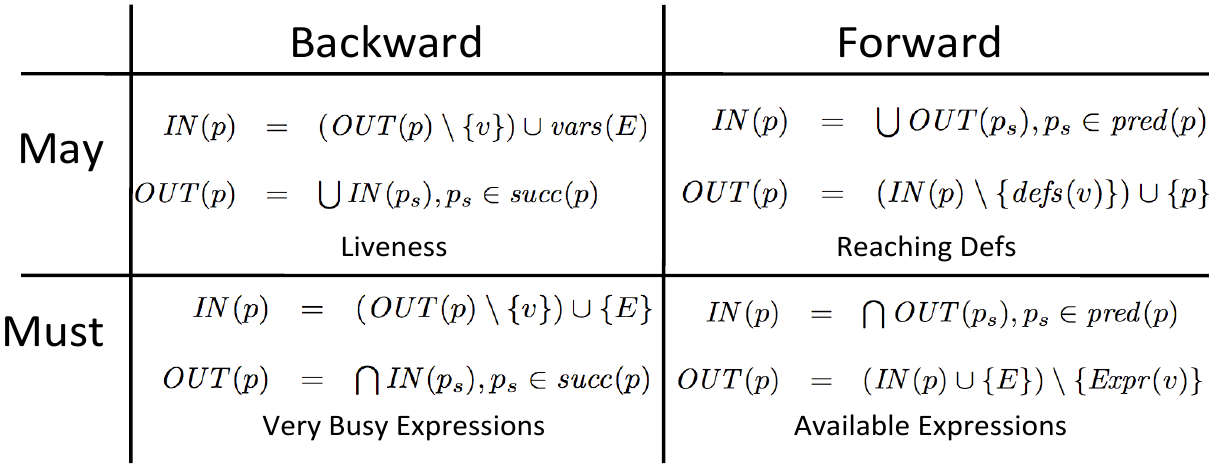
\includegraphics[scale=0.4]{res/image/commonalities_information}
  \caption{Fattori comuni delle varie analisi}
  \label{img:commonalities_information}
\end{figure}

\subsection{Funzione di trasferimento}
Un'analisi del flusso di dati fa qualche \textbf{interpretazione} del
programma, in modo da ottenere informazioni. Tuttavia la diretta
interpretazione della semantica concreta del nostro programma potrebbe
\textbf{non terminare mai}.

In modo da risolvere ci\'o si esegue un'\textit{interpretazione astratta}.
L'interpretazione viene applicata sulla semantica astratta presa data da una
\textit{funzione di trasferimento}.

A seconda che l'analisi si \textit{forward} o \textit{backward} la funzione di
trasferimento cambia:
\begin{align*}
& OUT[s] = f_s(IN[s]) {\color{red}\implies} \text{ Forward analysis} \\
& IN[s] = f_s(OUT[s]) {\color{red}\implies} \text{ Backward analysis}
\end{align*}

\subsection{Funzione di fusione}
\begin{definition}[Merging Function]
La funzione di fusione specifica cosa succede una volta che le informazioni
collidono.
\end{definition}

\begin{figure}[H]
  \centering
  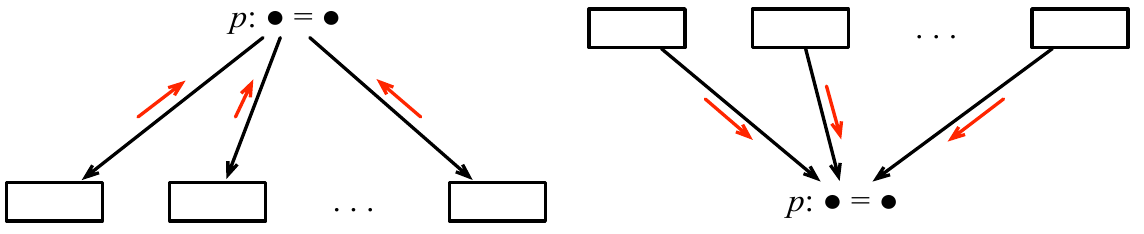
\includegraphics[scale=0.4]{res/image/merging_function}
  \caption{Funzione di fusione}
  \label{img:merging_function}
\end{figure}

La combinazione della funzione di trasferimento, funzione di fusione e (per
una certa entit\'a) l'inizializzazione di $IN$ e $OUT$ da noi la garanzia che
l'\textbf{interpretazione astratta termini}.
